\documentclass[12pt]{article}

%packages
%\usepackage{latexsym}
\usepackage{graphicx}
\usepackage{color}
\usepackage{amsmath}
\usepackage{dsfont}
\usepackage{placeins}
\usepackage{amssymb}
\usepackage{wasysym}
\usepackage{abstract}
\usepackage{hyperref}
\usepackage{etoolbox}
\usepackage{datetime}
\usepackage{xcolor}
\usepackage{alphalph}
\settimeformat{ampmtime}

%\usepackage{pstricks,pst-node,pst-tree}

%\usepackage{algpseudocode}
%\usepackage{amsthm}
%\usepackage{hyperref}
%\usepackage{mathrsfs}
%\usepackage{amsfonts}
%\usepackage{bbding}
%\usepackage{listings}
%\usepackage{appendix}
\usepackage[margin=1in]{geometry}
%\geometry{papersize={8.5in,11in},total={6.5in,9in}}
%\usepackage{cancel}
%\usepackage{algorithmic, algorithm}

\makeatletter
\def\maxwidth{ %
  \ifdim\Gin@nat@width>\linewidth
    \linewidth
  \else
    \Gin@nat@width
  \fi
}
\makeatother

\definecolor{fgcolor}{rgb}{0.345, 0.345, 0.345}
\newcommand{\hlnum}[1]{\textcolor[rgb]{0.686,0.059,0.569}{#1}}%
\newcommand{\hlstr}[1]{\textcolor[rgb]{0.192,0.494,0.8}{#1}}%
\newcommand{\hlcom}[1]{\textcolor[rgb]{0.678,0.584,0.686}{\textit{#1}}}%
\newcommand{\hlopt}[1]{\textcolor[rgb]{0,0,0}{#1}}%
\newcommand{\hlstd}[1]{\textcolor[rgb]{0.345,0.345,0.345}{#1}}%
\newcommand{\hlkwa}[1]{\textcolor[rgb]{0.161,0.373,0.58}{\textbf{#1}}}%
\newcommand{\hlkwb}[1]{\textcolor[rgb]{0.69,0.353,0.396}{#1}}%
\newcommand{\hlkwc}[1]{\textcolor[rgb]{0.333,0.667,0.333}{#1}}%
\newcommand{\hlkwd}[1]{\textcolor[rgb]{0.737,0.353,0.396}{\textbf{#1}}}%

\usepackage{framed}
\makeatletter
\newenvironment{kframe}{%
 \def\at@end@of@kframe{}%
 \ifinner\ifhmode%
  \def\at@end@of@kframe{\end{minipage}}%
  \begin{minipage}{\columnwidth}%
 \fi\fi%
 \def\FrameCommand##1{\hskip\@totalleftmargin \hskip-\fboxsep
 \colorbox{shadecolor}{##1}\hskip-\fboxsep
     % There is no \\@totalrightmargin, so:
     \hskip-\linewidth \hskip-\@totalleftmargin \hskip\columnwidth}%
 \MakeFramed {\advance\hsize-\width
   \@totalleftmargin\z@ \linewidth\hsize
   \@setminipage}}%
 {\par\unskip\endMakeFramed%
 \at@end@of@kframe}
\makeatother

\definecolor{shadecolor}{rgb}{.77, .77, .77}
\definecolor{messagecolor}{rgb}{0, 0, 0}
\definecolor{warningcolor}{rgb}{1, 0, 1}
\definecolor{errorcolor}{rgb}{1, 0, 0}
\newenvironment{knitrout}{}{} % an empty environment to be redefined in TeX

\usepackage{alltt}
\usepackage[T1]{fontenc}

\newcommand{\qu}[1]{``#1''}
\newcounter{probnum}
\setcounter{probnum}{1}

%create definition to allow local margin changes
\def\changemargin#1#2{\list{}{\rightmargin#2\leftmargin#1}\item[]}
\let\endchangemargin=\endlist 

%allow equations to span multiple pages
\allowdisplaybreaks

%define colors and color typesetting conveniences
\definecolor{gray}{rgb}{0.5,0.5,0.5}
\definecolor{black}{rgb}{0,0,0}
\definecolor{white}{rgb}{1,1,1}
\definecolor{blue}{rgb}{0.5,0.5,1}
\newcommand{\inblue}[1]{\color{blue}#1 \color{black}}
\definecolor{green}{rgb}{0.133,0.545,0.133}
\newcommand{\ingreen}[1]{\color{green}#1 \color{black}}
\definecolor{yellow}{rgb}{1,1,0}
\newcommand{\inyellow}[1]{\color{yellow}#1 \color{black}}
\definecolor{orange}{rgb}{0.9,0.649,0}
\newcommand{\inorange}[1]{\color{orange}#1 \color{black}}
\definecolor{red}{rgb}{1,0.133,0.133}
\newcommand{\inred}[1]{\color{red}#1 \color{black}}
\definecolor{purple}{rgb}{0.58,0,0.827}
\newcommand{\inpurple}[1]{\color{purple}#1 \color{black}}
\definecolor{backgcode}{rgb}{0.97,0.97,0.8}
\definecolor{Brown}{cmyk}{0,0.81,1,0.60}
\definecolor{OliveGreen}{cmyk}{0.64,0,0.95,0.40}
\definecolor{CadetBlue}{cmyk}{0.62,0.57,0.23,0}

%define new math operators
\DeclareMathOperator*{\argmax}{arg\,max~}
\DeclareMathOperator*{\argmin}{arg\,min~}
\DeclareMathOperator*{\argsup}{arg\,sup~}
\DeclareMathOperator*{\arginf}{arg\,inf~}
\DeclareMathOperator*{\convolution}{\text{\Huge{$\ast$}}}
\newcommand{\infconv}[2]{\convolution^\infty_{#1 = 1} #2}
%true functions

%%%% GENERAL SHORTCUTS

%shortcuts for pure typesetting conveniences
\newcommand{\bv}[1]{\boldsymbol{#1}}

%shortcuts for compound constants
\newcommand{\BetaDistrConst}{\dfrac{\Gamma(\alpha + \beta)}{\Gamma(\alpha)\Gamma(\beta)}}
\newcommand{\NormDistrConst}{\dfrac{1}{\sqrt{2\pi\sigma^2}}}

%shortcuts for conventional symbols
\newcommand{\tsq}{\tau^2}
\newcommand{\tsqh}{\hat{\tau}^2}
\newcommand{\sigsq}{\sigma^2}
\newcommand{\sigsqsq}{\parens{\sigma^2}^2}
\newcommand{\sigsqovern}{\dfrac{\sigsq}{n}}
\newcommand{\tausq}{\tau^2}
\newcommand{\tausqalpha}{\tau^2_\alpha}
\newcommand{\tausqbeta}{\tau^2_\beta}
\newcommand{\tausqsigma}{\tau^2_\sigma}
\newcommand{\betasq}{\beta^2}
\newcommand{\sigsqvec}{\bv{\sigma}^2}
\newcommand{\sigsqhat}{\hat{\sigma}^2}
\newcommand{\sigsqhatmlebayes}{\sigsqhat_{\text{Bayes, MLE}}}
\newcommand{\sigsqhatmle}[1]{\sigsqhat_{#1, \text{MLE}}}
\newcommand{\bSigma}{\bv{\Sigma}}
\newcommand{\bSigmainv}{\bSigma^{-1}}
\newcommand{\thetavec}{\bv{\theta}}
\newcommand{\thetahat}{\hat{\theta}}
\newcommand{\thetahatmle}{\hat{\theta}_{\mathrm{MLE}}}
\newcommand{\thetavechatmle}{\hat{\thetavec}_{\mathrm{MLE}}}
\newcommand{\muhat}{\hat{\mu}}
\newcommand{\musq}{\mu^2}
\newcommand{\muvec}{\bv{\mu}}
\newcommand{\muhatmle}{\muhat_{\text{MLE}}}
\newcommand{\lambdahat}{\hat{\lambda}}
\newcommand{\lambdahatmle}{\lambdahat_{\text{MLE}}}
\newcommand{\etavec}{\bv{\eta}}
\newcommand{\alphavec}{\bv{\alpha}}
\newcommand{\minimaxdec}{\delta^*_{\mathrm{mm}}}
\newcommand{\ybar}{\bar{y}}
\newcommand{\xbar}{\bar{x}}
\newcommand{\Xbar}{\bar{X}}
\newcommand{\phat}{\hat{p}}
\newcommand{\Phat}{\hat{P}}
\newcommand{\Zbar}{\bar{Z}}
\newcommand{\iid}{~{\buildrel iid \over \sim}~}
\newcommand{\inddist}{~{\buildrel ind \over \sim}~}
\newcommand{\approxdist}{~{\buildrel approx \over \sim}~}
\newcommand{\equalsindist}{~{\buildrel d \over =}~}
\newcommand{\loglik}[1]{\ell\parens{#1}}
\newcommand{\thetahatkminone}{\thetahat^{(k-1)}}
\newcommand{\thetahatkplusone}{\thetahat^{(k+1)}}
\newcommand{\thetahatk}{\thetahat^{(k)}}
\newcommand{\half}{\frac{1}{2}}
\newcommand{\third}{\frac{1}{3}}
\newcommand{\twothirds}{\frac{2}{3}}
\newcommand{\fourth}{\frac{1}{4}}
\newcommand{\fifth}{\frac{1}{5}}
\newcommand{\sixth}{\frac{1}{6}}

%shortcuts for vector and matrix notation
\newcommand{\A}{\bv{A}}
\newcommand{\At}{\A^T}
\newcommand{\Ainv}{\inverse{\A}}
\newcommand{\B}{\bv{B}}
\newcommand{\K}{\bv{K}}
\newcommand{\Kt}{\K^T}
\newcommand{\Kinv}{\inverse{K}}
\newcommand{\Kinvt}{(\Kinv)^T}
\newcommand{\M}{\bv{M}}
\newcommand{\Bt}{\B^T}
\newcommand{\Q}{\bv{Q}}
\newcommand{\Qt}{\Q^T}
\newcommand{\R}{\bv{R}}
\newcommand{\Rt}{\R^T}
\newcommand{\Z}{\bv{Z}}
\newcommand{\X}{\bv{X}}
\newcommand{\Xsub}{\X_{\text{(sub)}}}
\newcommand{\Xsubadj}{\X_{\text{(sub,adj)}}}
\newcommand{\I}{\bv{I}}
\newcommand{\Y}{\bv{Y}}
\newcommand{\sigsqI}{\sigsq\I}
\renewcommand{\P}{\bv{P}}
\newcommand{\Psub}{\P_{\text{(sub)}}}
\newcommand{\Pt}{\P^T}
\newcommand{\Pii}{P_{ii}}
\newcommand{\Pij}{P_{ij}}
\newcommand{\IminP}{(\I-\P)}
\newcommand{\Xt}{\bv{X}^T}
\newcommand{\XtX}{\Xt\X}
\newcommand{\XtXinv}{\parens{\Xt\X}^{-1}}
\newcommand{\XtXinvXt}{\XtXinv\Xt}
\newcommand{\XXtXinvXt}{\X\XtXinvXt}
\newcommand{\x}{\bv{x}}
\newcommand{\onevec}{\bv{1}}
\newcommand{\oneton}{1, \ldots, n}
\newcommand{\yoneton}{y_1, \ldots, y_n}
\newcommand{\yonetonorder}{y_{(1)}, \ldots, y_{(n)}}
\newcommand{\Yoneton}{Y_1, \ldots, Y_n}
\newcommand{\iinoneton}{i \in \braces{\oneton}}
\newcommand{\onetom}{1, \ldots, m}
\newcommand{\jinonetom}{j \in \braces{\onetom}}
\newcommand{\xoneton}{x_1, \ldots, x_n}
\newcommand{\Xoneton}{X_1, \ldots, X_n}
\newcommand{\xt}{\x^T}
\newcommand{\y}{\bv{y}}
\newcommand{\yt}{\y^T}
\renewcommand{\c}{\bv{c}}
\newcommand{\ct}{\c^T}
\newcommand{\tstar}{\bv{t}^*}
\renewcommand{\u}{\bv{u}}
\renewcommand{\v}{\bv{v}}
\renewcommand{\a}{\bv{a}}
\newcommand{\s}{\bv{s}}
\newcommand{\yadj}{\y_{\text{(adj)}}}
\newcommand{\xjadj}{\x_{j\text{(adj)}}}
\newcommand{\xjadjM}{\x_{j \perp M}}
\newcommand{\yhat}{\hat{\y}}
\newcommand{\yhatsub}{\yhat_{\text{(sub)}}}
\newcommand{\yhatstar}{\yhat^*}
\newcommand{\yhatstarnew}{\yhatstar_{\text{new}}}
\newcommand{\z}{\bv{z}}
\newcommand{\zt}{\z^T}
\newcommand{\bb}{\bv{b}}
\newcommand{\bbt}{\bb^T}
\newcommand{\bbeta}{\bv{\beta}}
\newcommand{\beps}{\bv{\epsilon}}
\newcommand{\bepst}{\beps^T}
\newcommand{\e}{\bv{e}}
\newcommand{\Mofy}{\M(\y)}
\newcommand{\KofAlpha}{K(\alpha)}
\newcommand{\ellset}{\mathcal{L}}
\newcommand{\oneminalph}{1-\alpha}
\newcommand{\SSE}{\text{SSE}}
\newcommand{\SSEsub}{\text{SSE}_{\text{(sub)}}}
\newcommand{\MSE}{\text{MSE}}
\newcommand{\RMSE}{\text{RMSE}}
\newcommand{\SSR}{\text{SSR}}
\newcommand{\SST}{\text{SST}}
\newcommand{\JSest}{\delta_{\text{JS}}(\x)}
\newcommand{\Bayesest}{\delta_{\text{Bayes}}(\x)}
\newcommand{\EmpBayesest}{\delta_{\text{EmpBayes}}(\x)}
\newcommand{\BLUPest}{\delta_{\text{BLUP}}}
\newcommand{\MLEest}[1]{\hat{#1}_{\text{MLE}}}

%shortcuts for Linear Algebra stuff (i.e. vectors and matrices)
\newcommand{\twovec}[2]{\bracks{\begin{array}{c} #1 \\ #2 \end{array}}}
\newcommand{\threevec}[3]{\bracks{\begin{array}{c} #1 \\ #2 \\ #3 \end{array}}}
\newcommand{\fivevec}[5]{\bracks{\begin{array}{c} #1 \\ #2 \\ #3 \\ #4 \\ #5 \end{array}}}
\newcommand{\twobytwomat}[4]{\bracks{\begin{array}{cc} #1 & #2 \\ #3 & #4 \end{array}}}
\newcommand{\threebytwomat}[6]{\bracks{\begin{array}{cc} #1 & #2 \\ #3 & #4 \\ #5 & #6 \end{array}}}

%shortcuts for conventional compound symbols
\newcommand{\thetainthetas}{\theta \in \Theta}
\newcommand{\reals}{\mathbb{R}}
\newcommand{\complexes}{\mathbb{C}}
\newcommand{\rationals}{\mathbb{Q}}
\newcommand{\integers}{\mathbb{Z}}
\newcommand{\naturals}{\mathbb{N}}
\newcommand{\forallninN}{~~\forall n \in \naturals}
\newcommand{\forallxinN}[1]{~~\forall #1 \in \reals}
\newcommand{\matrixdims}[2]{\in \reals^{\,#1 \times #2}}
\newcommand{\inRn}[1]{\in \reals^{\,#1}}
\newcommand{\mathimplies}{\quad\Rightarrow\quad}
\newcommand{\mathlogicequiv}{\quad\Leftrightarrow\quad}
\newcommand{\eqncomment}[1]{\quad \text{(#1)}}
\newcommand{\limitn}{\lim_{n \rightarrow \infty}}
\newcommand{\limitN}{\lim_{N \rightarrow \infty}}
\newcommand{\limitd}{\lim_{d \rightarrow \infty}}
\newcommand{\limitt}{\lim_{t \rightarrow \infty}}
\newcommand{\limitsupn}{\limsup_{n \rightarrow \infty}~}
\newcommand{\limitinfn}{\liminf_{n \rightarrow \infty}~}
\newcommand{\limitk}{\lim_{k \rightarrow \infty}}
\newcommand{\limsupn}{\limsup_{n \rightarrow \infty}}
\newcommand{\limsupk}{\limsup_{k \rightarrow \infty}}
\newcommand{\floor}[1]{\left\lfloor #1 \right\rfloor}
\newcommand{\ceil}[1]{\left\lceil #1 \right\rceil}

%shortcuts for environments
\newcommand{\beqn}{\vspace{-0.25cm}\begin{eqnarray*}}
\newcommand{\eeqn}{\end{eqnarray*}}
\newcommand{\bneqn}{\vspace{-0.25cm}\begin{eqnarray}}
\newcommand{\eneqn}{\end{eqnarray}}

%shortcuts for mini environments
\newcommand{\parens}[1]{\left(#1\right)}
\newcommand{\squared}[1]{\parens{#1}^2}
\newcommand{\tothepow}[2]{\parens{#1}^{#2}}
\newcommand{\prob}[1]{\mathbb{P}\parens{#1}}
\newcommand{\cprob}[2]{\prob{#1~|~#2}}
\newcommand{\littleo}[1]{o\parens{#1}}
\newcommand{\bigo}[1]{O\parens{#1}}
\newcommand{\Lp}[1]{\mathbb{L}^{#1}}
\renewcommand{\arcsin}[1]{\text{arcsin}\parens{#1}}
\newcommand{\prodonen}[2]{\bracks{\prod_{#1=1}^n #2}}
\newcommand{\mysum}[4]{\sum_{#1=#2}^{#3} #4}
\newcommand{\sumonen}[2]{\sum_{#1=1}^n #2}
\newcommand{\infsum}[2]{\sum_{#1=1}^\infty #2}
\newcommand{\infprod}[2]{\prod_{#1=1}^\infty #2}
\newcommand{\infunion}[2]{\bigcup_{#1=1}^\infty #2}
\newcommand{\infinter}[2]{\bigcap_{#1=1}^\infty #2}
\newcommand{\infintegral}[2]{\int^\infty_{-\infty} #2 ~\text{d}#1}
\newcommand{\supthetas}[1]{\sup_{\thetainthetas}\braces{#1}}
\newcommand{\bracks}[1]{\left[#1\right]}
\newcommand{\braces}[1]{\left\{#1\right\}}
\newcommand{\set}[1]{\left\{#1\right\}}
\newcommand{\abss}[1]{\left|#1\right|}
\newcommand{\norm}[1]{\left|\left|#1\right|\right|}
\newcommand{\normsq}[1]{\norm{#1}^2}
\newcommand{\inverse}[1]{\parens{#1}^{-1}}
\newcommand{\rowof}[2]{\parens{#1}_{#2\cdot}}

%shortcuts for functionals
\newcommand{\realcomp}[1]{\text{Re}\bracks{#1}}
\newcommand{\imagcomp}[1]{\text{Im}\bracks{#1}}
\newcommand{\range}[1]{\text{range}\bracks{#1}}
\newcommand{\colsp}[1]{\text{colsp}\bracks{#1}}
\newcommand{\rowsp}[1]{\text{rowsp}\bracks{#1}}
\newcommand{\tr}[1]{\text{tr}\bracks{#1}}
\newcommand{\rank}[1]{\text{rank}\bracks{#1}}
\newcommand{\proj}[2]{\text{Proj}_{#1}\bracks{#2}}
\newcommand{\projcolspX}[1]{\text{Proj}_{\colsp{\X}}\bracks{#1}}
\newcommand{\median}[1]{\text{median}\bracks{#1}}
\newcommand{\mean}[1]{\text{mean}\bracks{#1}}
\newcommand{\dime}[1]{\text{dim}\bracks{#1}}
\renewcommand{\det}[1]{\text{det}\bracks{#1}}
\newcommand{\expe}[1]{\mathbb{E}\bracks{#1}}
\newcommand{\expeabs}[1]{\expe{\abss{#1}}}
\newcommand{\expesub}[2]{\mathbb{E}_{#1}\bracks{#2}}
\newcommand{\indic}[1]{\mathds{1}_{#1}}
\newcommand{\var}[1]{\mathbb{V}\text{ar}\bracks{#1}}
\newcommand{\cov}[2]{\mathbb{C}\text{ov}\bracks{#1, #2}}
\newcommand{\corr}[2]{\text{Corr}\bracks{#1, #2}}
\newcommand{\se}[1]{\mathbb{S}\text{E}\bracks{#1}}
\newcommand{\seest}[1]{\hat{\mathbb{S}\text{E}}\bracks{#1}}
\newcommand{\bias}[1]{\text{Bias}\bracks{#1}}
\newcommand{\derivop}[2]{\dfrac{\text{d}}{\text{d} #1}\bracks{#2}}
\newcommand{\partialop}[2]{\dfrac{\partial}{\partial #1}\bracks{#2}}
\newcommand{\secpartialop}[2]{\dfrac{\partial^2}{\partial #1^2}\bracks{#2}}
\newcommand{\mixpartialop}[3]{\dfrac{\partial^2}{\partial #1 \partial #2}\bracks{#3}}

%shortcuts for functions
\renewcommand{\exp}[1]{\mathrm{exp}\parens{#1}}
\renewcommand{\cos}[1]{\text{cos}\parens{#1}}
\renewcommand{\sin}[1]{\text{sin}\parens{#1}}
\newcommand{\sign}[1]{\text{sign}\parens{#1}}
\newcommand{\are}[1]{\mathrm{ARE}\parens{#1}}
\newcommand{\natlog}[1]{\ln\parens{#1}}
\newcommand{\oneover}[1]{\frac{1}{#1}}
\newcommand{\overtwo}[1]{\frac{#1}{2}}
\newcommand{\overn}[1]{\frac{#1}{n}}
\newcommand{\oneoversqrt}[1]{\oneover{\sqrt{#1}}}
\newcommand{\sqd}[1]{\parens{#1}^2}
\newcommand{\loss}[1]{\ell\parens{\theta, #1}}
\newcommand{\losstwo}[2]{\ell\parens{#1, #2}}
\newcommand{\cf}{\phi(t)}

%English language specific shortcuts
\newcommand{\ie}{\textit{i.e.} }
\newcommand{\AKA}{\textit{AKA} }
\renewcommand{\iff}{\textit{iff}}
\newcommand{\eg}{\textit{e.g.} }
\newcommand{\st}{\textit{s.t.} }
\newcommand{\wrt}{\textit{w.r.t.} }
\newcommand{\mathst}{~~\text{\st}~~}
\newcommand{\mathand}{~~\text{and}~~}
\newcommand{\ala}{\textit{a la} }
\newcommand{\ppp}{posterior predictive p-value}
\newcommand{\dd}{dataset-to-dataset}

%shortcuts for distribution titles
\newcommand{\logistic}[2]{\mathrm{Logistic}\parens{#1,\,#2}}
\newcommand{\bernoulli}[1]{\mathrm{Bernoulli}\parens{#1}}
\newcommand{\betanot}[2]{\mathrm{Beta}\parens{#1,\,#2}}
\newcommand{\stdbetanot}{\betanot{\alpha}{\beta}}
\newcommand{\multnormnot}[3]{\mathcal{N}_{#1}\parens{#2,\,#3}}
\newcommand{\normnot}[2]{\mathcal{N}\parens{#1,\,#2}}
\newcommand{\classicnormnot}{\normnot{\mu}{\sigsq}}
\newcommand{\stdnormnot}{\normnot{0}{1}}
\newcommand{\uniformdiscrete}[1]{\mathrm{Uniform}\parens{\braces{#1}}}
\newcommand{\uniform}[2]{\mathrm{U}\parens{#1,\,#2}}
\newcommand{\stduniform}{\uniform{0}{1}}
\newcommand{\geometric}[1]{\mathrm{Geometric}\parens{#1}}
\newcommand{\hypergeometric}[3]{\mathrm{Hypergeometric}\parens{#1,\,#2,\,#3}}
\newcommand{\exponential}[1]{\mathrm{Exp}\parens{#1}}
\newcommand{\gammadist}[2]{\mathrm{Gamma}\parens{#1, #2}}
\newcommand{\poisson}[1]{\mathrm{Poisson}\parens{#1}}
\newcommand{\binomial}[2]{\mathrm{Binomial}\parens{#1,\,#2}}
\newcommand{\negbin}[2]{\mathrm{NegBin}\parens{#1,\,#2}}
\newcommand{\rayleigh}[1]{\mathrm{Rayleigh}\parens{#1}}
\newcommand{\multinomial}[2]{\mathrm{Multinomial}\parens{#1,\,#2}}
\newcommand{\gammanot}[2]{\mathrm{Gamma}\parens{#1,\,#2}}
\newcommand{\cauchynot}[2]{\text{Cauchy}\parens{#1,\,#2}}
\newcommand{\invchisqnot}[1]{\text{Inv}\chisq{#1}}
\newcommand{\invscaledchisqnot}[2]{\text{ScaledInv}\ncchisq{#1}{#2}}
\newcommand{\invgammanot}[2]{\text{InvGamma}\parens{#1,\,#2}}
\newcommand{\chisq}[1]{\chi^2_{#1}}
\newcommand{\ncchisq}[2]{\chi^2_{#1}\parens{#2}}
\newcommand{\ncF}[3]{F_{#1,#2}\parens{#3}}

%shortcuts for PDF's of common distributions
\newcommand{\logisticpdf}[3]{\oneover{#3}\dfrac{\exp{-\dfrac{#1 - #2}{#3}}}{\parens{1+\exp{-\dfrac{#1 - #2}{#3}}}^2}}
\newcommand{\betapdf}[3]{\dfrac{\Gamma(#2 + #3)}{\Gamma(#2)\Gamma(#3)}#1^{#2-1} (1-#1)^{#3-1}}
\newcommand{\normpdf}[3]{\frac{1}{\sqrt{2\pi#3}}\exp{-\frac{1}{2#3}(#1 - #2)^2}}
\newcommand{\normpdfvarone}[2]{\dfrac{1}{\sqrt{2\pi}}e^{-\half(#1 - #2)^2}}
\newcommand{\chisqpdf}[2]{\dfrac{1}{2^{#2/2}\Gamma(#2/2)}\; {#1}^{#2/2-1} e^{-#1/2}}
\newcommand{\invchisqpdf}[2]{\dfrac{2^{-\overtwo{#1}}}{\Gamma(#2/2)}\,{#1}^{-\overtwo{#2}-1}  e^{-\oneover{2 #1}}}
\newcommand{\exponentialpdf}[2]{#2\exp{-#2#1}}
\newcommand{\poissonpdf}[2]{\dfrac{e^{-#1} #1^{#2}}{#2!}}
\newcommand{\binomialpdf}[3]{\binom{#2}{#1}#3^{#1}(1-#3)^{#2-#1}}
\newcommand{\rayleighpdf}[2]{\dfrac{#1}{#2^2}\exp{-\dfrac{#1^2}{2 #2^2}}}
\newcommand{\gammapdf}[3]{\dfrac{#3^#2}{\Gamma\parens{#2}}#1^{#2-1}\exp{-#3 #1}}
\newcommand{\cauchypdf}[3]{\oneover{\pi} \dfrac{#3}{\parens{#1-#2}^2 + #3^2}}
\newcommand{\Gammaf}[1]{\Gamma\parens{#1}}

%shortcuts for miscellaneous typesetting conveniences
\newcommand{\notesref}[1]{\marginpar{\color{gray}\tt #1\color{black}}}

%%%% DOMAIN-SPECIFIC SHORTCUTS

%Real analysis related shortcuts
\newcommand{\zeroonecl}{\bracks{0,1}}
\newcommand{\forallepsgrzero}{\forall \epsilon > 0~~}
\newcommand{\lessthaneps}{< \epsilon}
\newcommand{\fraccomp}[1]{\text{frac}\bracks{#1}}

%Bayesian related shortcuts
\newcommand{\yrep}{y^{\text{rep}}}
\newcommand{\yrepisq}{(\yrep_i)^2}
\newcommand{\yrepvec}{\bv{y}^{\text{rep}}}


%Probability shortcuts
\newcommand{\SigField}{\mathcal{F}}
\newcommand{\ProbMap}{\mathcal{P}}
\newcommand{\probtrinity}{\parens{\Omega, \SigField, \ProbMap}}
\newcommand{\convp}{~{\buildrel p \over \rightarrow}~}
\newcommand{\convLp}[1]{~{\buildrel \Lp{#1} \over \rightarrow}~}
\newcommand{\nconvp}{~{\buildrel p \over \nrightarrow}~}
\newcommand{\convae}{~{\buildrel a.e. \over \longrightarrow}~}
\newcommand{\convau}{~{\buildrel a.u. \over \longrightarrow}~}
\newcommand{\nconvau}{~{\buildrel a.u. \over \nrightarrow}~}
\newcommand{\nconvae}{~{\buildrel a.e. \over \nrightarrow}~}
\newcommand{\convd}{~{\buildrel \mathcal{D} \over \rightarrow}~}
\newcommand{\nconvd}{~{\buildrel \mathcal{D} \over \nrightarrow}~}
\newcommand{\withprob}{~~\text{w.p.}~~}
\newcommand{\io}{~~\text{i.o.}}

\newcommand{\Acl}{\bar{A}}
\newcommand{\ENcl}{\bar{E}_N}
\newcommand{\diam}[1]{\text{diam}\parens{#1}}

\newcommand{\taua}{\tau_a}

\newcommand{\myint}[4]{\int_{#2}^{#3} #4 \,\text{d}#1}
\newcommand{\laplacet}[1]{\mathscr{L}\bracks{#1}}
\newcommand{\laplaceinvt}[1]{\mathscr{L}^{-1}\bracks{#1}}
\renewcommand{\min}[1]{\text{min}\braces{#1}}
\renewcommand{\max}[1]{\text{max}\braces{#1}}

\newcommand{\Vbar}[1]{\bar{V}\parens{#1}}
\newcommand{\expnegrtau}{\exp{-r\tau}}

%%% problem typesetting
\definecolor{darkgrey}{rgb}{0.10,0.10,0.9}

\newcommand{\problem}[1]{\noindent \colorbox{black}{{\color{yellow} \large{\textsf{\textbf{Problem \arabic{probnum}}}}~}} \addtocounter{probnum}{1} \vspace{0.2cm} \\ \iftoggle{professormode}{}{\color{darkgrey}} #1}

\newcommand{\easysubproblem}[1]{\ingreen{\item} \iftoggle{professormode}{}{\color{darkgrey}} [easy] #1 \color{black} }
\newcommand{\intermediatesubproblem}[1]{\inorange{\item} \iftoggle{professormode}{}{\color{darkgrey}} [harder] #1 \color{black} }
\newcommand{\hardsubproblem}[1]{\inred{\item} \iftoggle{professormode}{}{\color{darkgrey}} [difficult] #1 \color{black} }
\newcommand{\extracreditsubproblem}[1]{\inpurple{\item} \iftoggle{professormode}{}{\color{darkgrey}} [E.C.] #1 \color{black} }


\newcommand{\spc}[1]{\iftoggle{professormode}{\\ \vspace{#1cm}}{\\ \vspace{-0.3cm}}}

\makeatletter
\newalphalph{\alphmult}[mult]{\@alph}{26}
\renewcommand{\labelenumi}{(\alphmult{\value{enumi}})}

\newcommand{\support}[1]{\text{Supp}\bracks{#1}}
\newcommand{\mode}[1]{\text{Mode}\bracks{#1}}
\newcommand{\IQR}[1]{\text{IQR}\bracks{#1}}
\newcommand{\quantile}[2]{\text{Quantile}\bracks{#1,\,#2}}
\usepackage{graphicx}


\newtoggle{professormode}



\title{MATH 342W / 650.4 Spring \the\year~Homework \#2}

\author{Loyd Flores.
} %STUDENTS: write your name here

\iftoggle{professormode}{
\date{Due 11:59PM Feb 25, \the\year \\ \vspace{0.5cm} \small (this document last updated \currenttime~on \today)}
}

\renewcommand{\abstractname}{Instructions and Philosophy}

\begin{document}
\maketitle

\iftoggle{professormode}{
\begin{abstract}
The path to success in this class is to do many problems. Unlike other courses, exclusively doing reading(s) will not help. Coming to lecture is akin to watching workout videos; thinking about and solving problems on your own is the actual ``working out.''  Feel free to \qu{work out} with others; \textbf{I want you to work on this in groups.}

Reading is still \textit{required}. You should be googling and reading about all the concepts introduced in class online. This is your responsibility to supplement in-class with your own readings.

The problems below are color coded: \ingreen{green} problems are considered \textit{easy} and marked \qu{[easy]}; \inorange{yellow} problems are considered \textit{intermediate} and marked \qu{[harder]}, \inred{red} problems are considered \textit{difficult} and marked \qu{[difficult]} and \inpurple{purple} problems are extra credit. The \textit{easy} problems are intended to be ``giveaways'' if you went to class. Do as much as you can of the others; I expect you to at least attempt the \textit{difficult} problems. 

This homework is worth 100 points but the point distribution will not be determined until after the due date. See syllabus for the policy on late homework.

Up to 7 points are given as a bonus if the homework is typed using \LaTeX. Links to instaling \LaTeX~and program for compiling \LaTeX~is found on the syllabus. You are encouraged to use \url{overleaf.com}. If you are handing in homework this way, read the comments in the code; there are two lines to comment out and you should replace my name with yours and write your section. The easiest way to use overleaf is to copy the raw text from hwxx.tex and preamble.tex into two new overleaf tex files with the same name. If you are asked to make drawings, you can take a picture of your handwritten drawing and insert them as figures or leave space using the \qu{$\backslash$vspace} command and draw them in after printing or attach them stapled.

The document is available with spaces for you to write your answers. If not using \LaTeX, print this document and write in your answers. I do not accept homeworks which are \textit{not} on this printout. Keep this first page printed for your records.

\end{abstract}

\thispagestyle{empty}
\vspace{1cm}
NAME: Loyd Flores \line(1,0){380}
\clearpage
}

\problem{These are questions about Silver's book, chapter 2, 3.  Answer the questions using notation from class (i.e. $t ,f, g, h^*, \delta, \epsilon, e, t, z_1, \ldots, z_t, \mathbb{D}, \mathcal{H}, \mathcal{A}, \mathcal{X}, \mathcal{Y}, X, y, n, p, x_{\cdot 1}, \ldots, x_{\cdot p}, x_{1 \cdot}, \ldots, x_{n \cdot}$, etc).}


\begin{enumerate}

\intermediatesubproblem{If one's goal is to fit a model for a phenomenon $y$, what is the difference between the approaches of the hedgehog and the fox? Connecting this to the modeling framework should really make you think about what Tetlock's observation means for political and historical phenomena.} \\
\textbf{Answer: } \\
Philip Tetlock observed that experts' predictions varied, with some performing better than others. He classified these experts into two groups: \textit{Hedgehogs and Foxes}. Hedgehogs tend to approach modeling phenomena with rigidity, similar to hunting one large prey, relying on a single overarching theory to explain phenomena. They often struggle to separate their own biases from their analysis, leading to a fusion of facts and values. In terms of fitting a model, hedgehogs tend to over-fit. In contrast, Foxes possess a multidisciplinary approach, considering many diverse ideas and embracing uncertainty. They recognize the limitations of a single theory and adapt their views based on new information. Tetlock's findings emphasize the importance of open-mindedness and consideration of different perspectives, particularly in fields such as politics, history, and model development. Fox-like thinkers adjust their views based on new information and are better equipped to understand complex issues, while Hedgehog thinkers remain rigid and oversimplify problems, allowing biases to influence their conclusions. Recognizing these different thinking styles helps us strive for a clearer and more truthful understanding of the world as it is, rather than how we wish to perceive it.

\easysubproblem{Why did Harry Truman like hedgehogs? Are there a lot of people that think this way?} \\
\textbf{Answer: } \\

Foxes face challenges in various domains such as television, business, and politics. Their modest predictions regarding complex issues are often misinterpreted as a lack of confidence and conviction. However, this modesty stems from Foxes' acknowledgment of the uncertainties and complexities inherent in such problems. Foxes frustrate Truman due to their inability to provide straightforward answers. Truman's preference for Hedgehog-like responses, evident in his impatience with his Fox-minded administration members, reflects a desire for simplified solutions. It appears that Truman prioritizes speed over quality, seeking quick, definitive answers, even if they may be incorrect. Foxes, on the other hand, are perceived as too slow and hesitant, as they prioritize thorough analysis over hasty conclusions.




\hardsubproblem{Why is it that the more education one acquires, the less accurate one's predictions become?} \\
\textbf{Answer: } \\ 

This holds particularly true for individuals with a Hedgehog-like mindset. When presented with more facts, there arises a greater potential for these facts to be twisted and manipulated to align with existing biases. This merging of facts and values becomes a significant concern. However, if one can effectively separate biases from the analysis, additional information can indeed prove beneficial in comprehending the intricacies of data relationships.

\easysubproblem{Why are probabilistic classifiers (i.e. algorithms that output functions that return probabilities) better than vanilla classifiers (i.e. algorithms that only return the class label)? We will move in this direction in class soon.} \\
\textbf{Answer: }

In my view, \textit{probabilistic classifiers} outperform \textit{vanilla classifiers} because they don't just predict the best possible class, which can only result in a binary outcome of right or wrong. Instead, probabilistic classifiers predict the probabilities associated with each potential class. This is particularly advantageous when uncertainty is significant because the model not only makes predictions but also provides information about its confidence level in those predictions. This feature empowers engineers with actionable insights, enabling them to make necessary adjustments to the model or take further steps in data exploration.

\easysubproblem{What algorithm that we studied in class is PECOTA most similar to?} \\
\textbf{Answer: } \\ 

PECOTA appears quite similar to the NN or KNN (Nearest Neighbor or K Nearest Neighbor) algorithm. PECOTA employs a concept known as \textit{similarity scores}, designed to evaluate the statistical similarity between the career statistics of any two major-league baseball players. This concept mirrors how NN or KNN functions in theory. Instead of similarity scores, NN/KNN uses a distance function to determine the closest data point or class, which is then used to make a prediction. Similarly, PECOTA groups together players with the closest similarity scores and predicts a player's career trajectory based on the players they are associated with. \\

\easysubproblem{Is baseball performance as a function of age a linear model? Discuss.} \\ 
\textbf{Answer: } \\ 
In a way, you could argue yes, but ultimately, it is not. If you frame the problem as predicting whether someone is good with a yes/no outcome and use age as the main feature, you would need to determine that age and set it as a threshold for the model to predict player performance solely based on age. This approach might make the data appear linearly separable, but it would be an oversimplification. There are numerous factors influencing a baseball player's performance, such as the current environment, injuries, and mental maturity. With such complexity in the data, a linear model would struggle to capture the relationships and would oversimplify the issue at hand.


\intermediatesubproblem{How can baseball scouts do better than a prediction system like PECOTA?} \\ 
\textbf{Answer: } \\ 
Both scouts and PECOTA have the ability to analyze statistical information, such as batting average. A model like PECOTA may be more efficient and accurate than a scout in terms of statistical computation and the elimination of existing biases. However, scouts have an advantage in accessing additional information that models do not have access to. Scouts can gather more information over time, such as the actual speed of pitches and hits in real-time, rather than solely relying on available statistical data. This multi-source information enables scouts to make more informed decisions compared to models, which can only predict based on available data.

\intermediatesubproblem{Why hasn't anyone (at the time of the writing of Silver's book) taken advantage of Pitch f/x data to predict future success?} \\ 
\textbf{Answer: } \\ 

To my understanding, at the time of the publication of Silver's book, Pitch f/x was relatively new to the game, introducing many new measurable metrics such as the horizontal and vertical movement of a pitched ball. These metrics could be utilized as features to enhance our models' ability to predict a target 'y'. However, at that time, these metrics were more applicable in the scouting realm, as people were still understanding the relationships they would create and their correlation to the target 'y'. Once people figure out how to effectively utilize this data, it could be applied in the realm of forecasting. However, simply inserting this newfound data into our models might produce garbage or overfit our model, as it would introduce unnecessary noise. To conclude like stated in Silver's introduction it takes time for people to utilize newfound data, like the invention of the printing press it took another 300 years for its effects to show. In time people will learn how to utilize the new data and produce more accurate and descriptive models. \\ \\ \\ \\
\\


\end{enumerate}



\problem{These are questions about the SVM.}

\begin{enumerate}

\easysubproblem{State the hypothesis set $\mathcal{H}$ inputted into the support vector machine algorithm. Is it different than the $\mathcal{H}$ used for $\mathcal{A}$ = perceptron learning algorithm?} \\ 
\spc{Answer: } \\
The objectives of the Perceptron Learning Algorithm and Support Vector Machines are quite similar; both aim to draw a line that linearly separates our data. However, their approaches differ. Support vectors act as balloons that can be enlarged, guiding and enhancing flexibility in finding the optimal hyperplane by maximizing the margin, or the space between the hyperplane and the data points. In contrast, the Perceptron focuses solely on adjusting weights to achieve the best line that separates the classes without margin optimization. Despite this distinction, both algorithms share an H consisting of all linear functions. However, SVM's H comprises a set of linear functions representing hyperplanes supported by support vectors, while the Perceptron's 
H consists of linear functions that determine the best line by adjusting weights.







\extracreditsubproblem{Prove the max-margin linearly separable SVM converges. State all assumptions. Write it on a separate page.} \\ 
\spc{Answer: } \\ 
Assumptions: \\
1. D is linearly separable, therefore there exists a hyperplane that separates the data points \\
2. There exists an optimization software / formula \\
3. Iteratively our optimization formula will continuously adjust the parameters (weights and intercept) to find the best hyperplane \\
4. Since data is linearly separable SVM will always converge to find an h.\\


\hardsubproblem{Let $\mathcal{Y} = \braces{-1,1}$. Rederive the cost function whose minimization yields the SVM line in the linearly separable case. }\spc{20}

\easysubproblem{Given your answer to (c) rederive the cost function using the \qu{soft margin} i.e. the hinge loss plus the term with the hyperparameter $\lambda$. This is marked easy since there is just one change from the expression given in class.}\spc{4}

\end{enumerate}



\problem{These are questions are about the $k$ nearest neighbors (KNN) algorithm.}

\begin{enumerate}

\easysubproblem{Describe how the algorithm works. Is $k$ a \qu{hyperparameter}?} \\
\textbf{Answer: } \\ 
The K nearest neighbor algorithm works by identifying the closest data points and classifying them together. When a model employs KNN, the prediction is determined by the class associated with the nearest data point. Different distance functions, such as Manhattan and Euclidean distance, are used to calculate the distance. K serves as a hyperparameter of KNN, representing the number of neighbors the model will consider when grouping points together. The choice of K significantly impacts the model's performance, and it is the engineer's responsibility to determine an appropriate value. Maximizing K may result in overfitting, as everyone becomes a neighbor, while selecting a K that is too low may lead to inaccurate assumptions. 

\hardsubproblem{[MA] Assuming $\mathcal{A} = $ KNN, describe the input $\mathcal{H}$ as best as you can.} \\ 
\textbf{Answer: } \\ 
For example we have a simple 2-Dimensional Dataset and each data point will either only red or blue. 
H in this case will be composed of functions that all possible classifications based on the nearest neighbor provided by the Distance Function selected. In summary H encompases all possible classifications determined by class of its neighbor (red or blue), that changes depending on the hyper-parameter K selected.

\easysubproblem{When predicting on $\mathbb{D}$ with $k=1$, why should there be zero error? Is this a good estimate of future error when new data comes in? (Error in the future is called \emph{generalization error} and we will be discussing this later in the semester).} \\
\textbf{Answer: } \\ 
When the hyperparameter k is set to 1, it means we're considering only one neighbor. The closest neighbor will then be the data point itself. In essence, you're grouping the data points by themselves. You obtain a 0 error because the model predicts each data point will be grouped with itself as it's the closest one. This is not a good estimate because it's not entirely true that you obtained a model that can't make mistakes. It will perform poorly on unseen data and will often misclassify data points into incorrect classes.


\end{enumerate}

\problem{These are questions about the linear model with $p=1$.}

\begin{enumerate}

\easysubproblem{What does $\mathbb{D}$ look like in the linear model with $p=1$? What is $\mathcal{X}$? What is $\mathcal{Y}$?} \\
\textbf{Answer: } \\ 
When `p` = 1 in linear models it means that there is only one feature being used to explain the response or the target variable. This then assumes the relationship between feature and target is linear. The model then assumes that there is a straigh-line relationship and the goal is to find the best fitting line that describes their relationship. For example in a regression problem the number of rooms may determine house price or in a classification problem that line may separate data by class. \\ \\ \\ \\ \\


\easysubproblem{Consider the line fit using the ordinary least squares (OLS) algorithm. Prove that the point $<\xbar, \ybar>$ is on this line. Use the formulas we derived in class.} \\ 
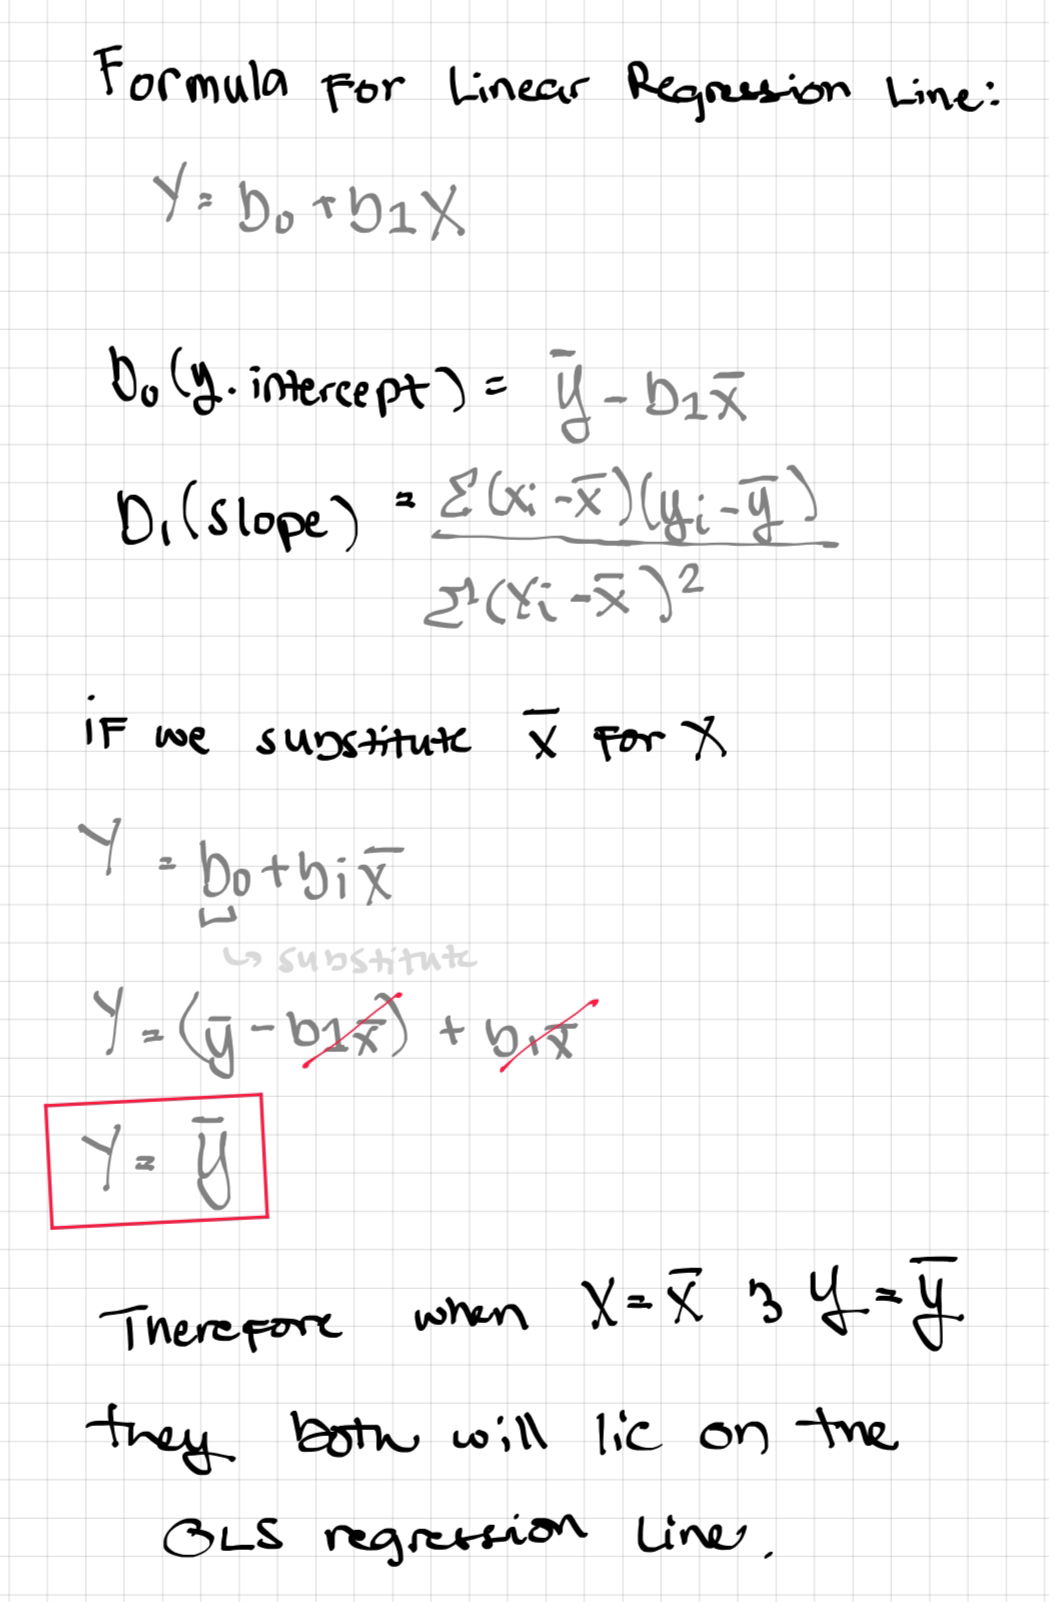
\includegraphics[width=12cm, keepaspectratio]{4b.png} \\ \\  \\ \\ \\ \\ 


\intermediatesubproblem{Consider the line fit using OLS. Prove that the average prediction $\hat{y}_i := g(x_i)$ for $x_i \in \mathbb{D}$ is $\ybar$.} \\ 
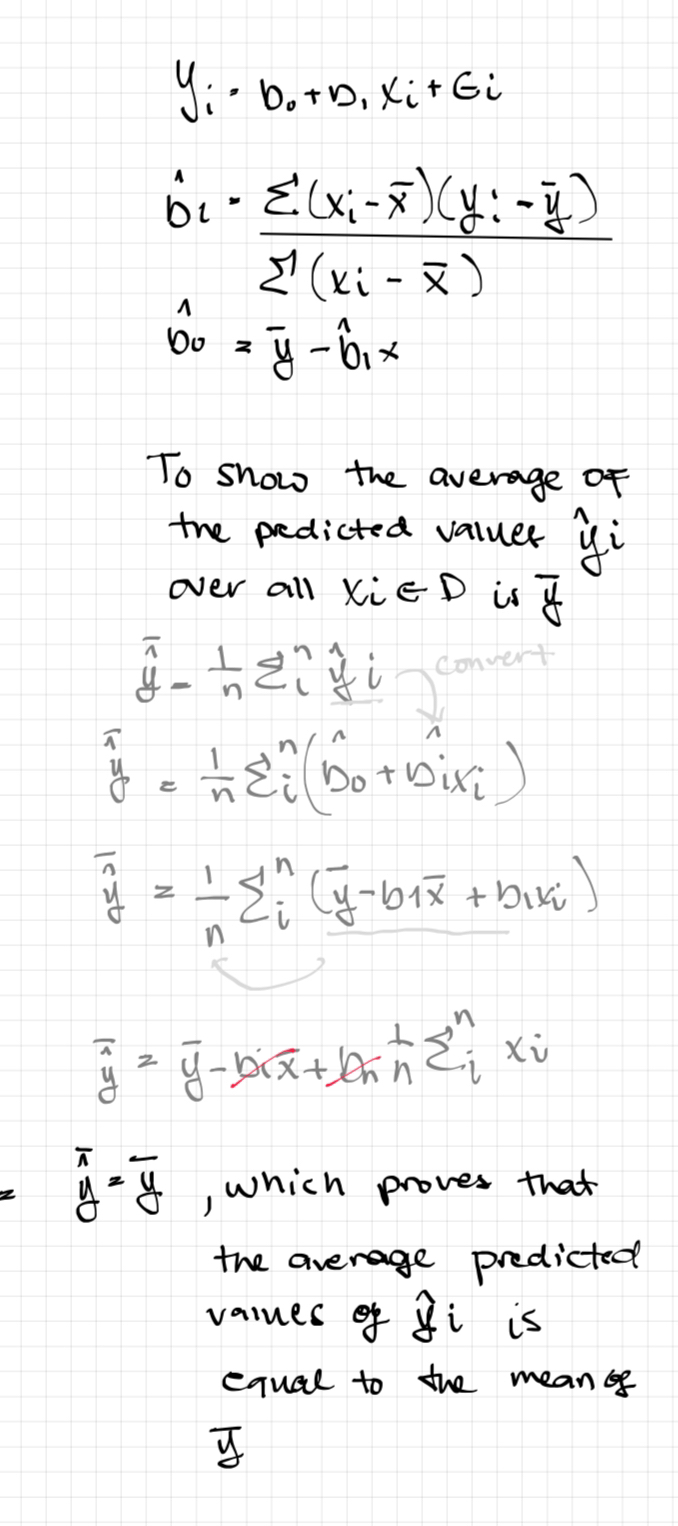
\includegraphics[width=9cm, keepaspectratio]{4c.png} \\ \\ \\


\intermediatesubproblem{Consider the line fit using OLS. Prove that the average residual $e_i$ is 0 over $\mathbb{D}$.} \\ 
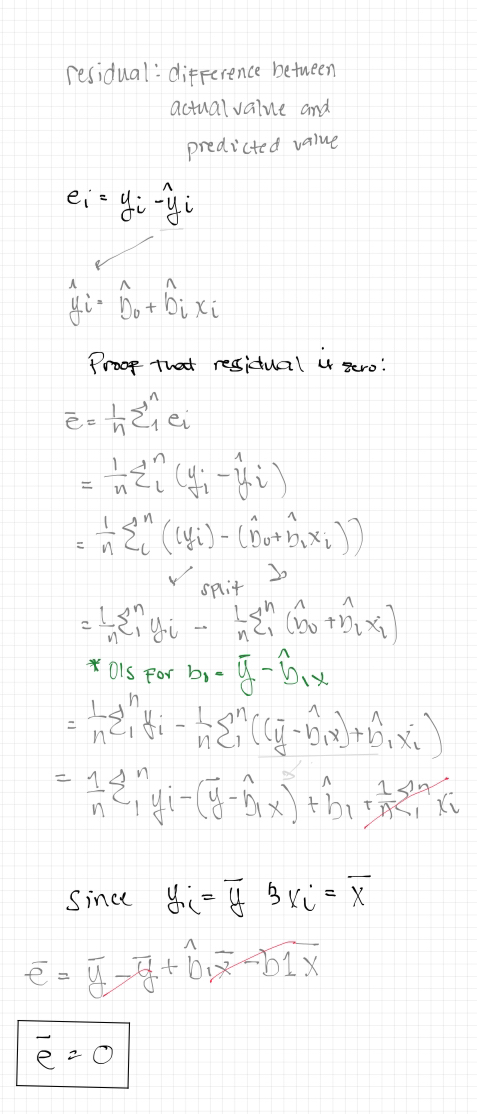
\includegraphics[width=9cm, keepaspectratio]{4d.png} \\ 

\intermediatesubproblem{Why is the RMSE usually a better indicator of predictive performance than $R^2$? Discuss in English.} \\ 
\textbf{Answer: } \\

For instance, when attempting to predict a car's price based on features such as the number of doors, engine size, etc., RMSE provides a value in the same unit as the response. This tells us, on average, how much our predictions deviate from the actual prices. If the RMSE is \$1,000, it indicates that the average error in the model's predicted price is \$1,000. In contrast, $R^{2}$ will return a statistic like 0.80 or 80\%, suggesting that this proportion of variability in car prices is accounted for by the factors in the model. The remaining 20\% might be due to factors not included in the model. In this example, RMSE is more informative because it returns a value in the same unit as the response, making it easier to understand the extent of our deviations. On the other hand, $R^{2}$ yields a dimensionless statistic that explains the proportion of variance in the dependent variable but does not directly indicate the magnitude of the errors. \\ \\ \\ \\ \\ \\ \\ \\ \\ \\ \\ \\ \\ \\ \\ \\ \\ \\ \\ \\ \\ \\ \\ \\ \\ \\ \\ \\ \\


\intermediatesubproblem{$R^2$ is commonly interpreted as \qu{proportion of the variance explained by the model} and proportions are constrained to the interval $\zeroonecl$. While it is true that $R^2 \leq 1$ for all models, it is not true that $R^2 \geq 0$ for all models. Construct an explicit example $\mathbb{D}$ and create a linear model $g(x) = w_0 + w_1 x$ whose $R^2 < 0$.} \\ 
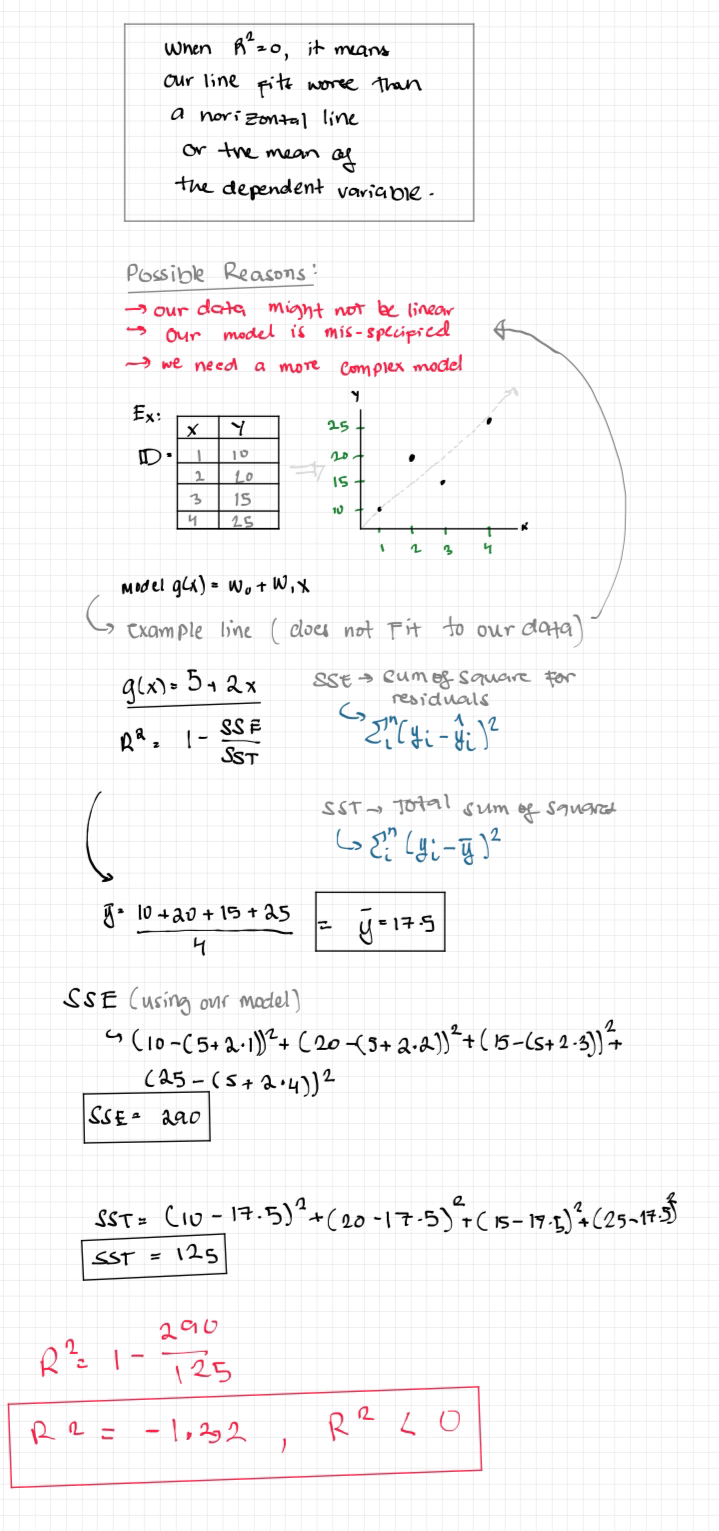
\includegraphics[width=8cm, keepaspectratio]{4f.png} \\ 


\hardsubproblem{You are given $\mathbb{D}$ with $n$ training points $<x_i, y_i>$ but now you are also given a set of weights $\bracks{w_1~w_2~ \ldots ~w_n}$ which indicate how costly the error is for each of the $i$ points. Rederive the least squares estimates $b_0$ and $b_1$ under this situation. Note that these estimates are called the \emph{weighted least squares regression} estimates. This variant $\mathcal{A}$ on OLS has a number of practical uses, especially in Economics. No need to simplify your answers like I did in class (i.e. you can leave in ugly sums).}\spc{12.5}


\intermediatesubproblem{Interpret the ugly sums in the $b_0$ and $b_1$ you derived above and compare them to the $b_0$ and $b_1$ estimates in OLS. Does it make sense each term should be altered in this matter given your goal in the weighted least squares?}\spc{5}


%\hardsubproblem{[MA] In class we talked about $x_{raw} \in \braces{\text{red}, \text{green}}$ and the OLS model was the sample average of the inputted $x$ where $b_0 = \ybar_r$ and $b_1 = \ybar_g - \ybar_r$. Reparameterize $\mathcal{H} = \braces{w_1\indic{x_{raw} =~\text{red}}  + w_2 \indic{x_{raw} =~\text{green}}~:~ w_1, w_2 \in \reals}$ and prove that the OLS estimates are $b_1 = \ybar_r$ and $b_2 = \ybar_g$.}\spc{20}

\extracreditsubproblem{In class we talked about $x_{raw} \in \braces{\text{red}, \text{green}}$ and the OLS model was the sample average of the inputted $x$. Imagine if you have the additional constraint that $x_{raw}$ is ordinal e.g. $x_{raw} \in \braces{\text{low}, \text{high}}$ and you were forced to have a model where $g$(low) $\leq$ $g$(high). Write about an algorithm $\mathcal{A}$ that can solve this problem.}\spc{10}

\end{enumerate}
\newpage
\problem{These are questions about association and correlation.}



\begin{enumerate}

\easysubproblem{Give an example of two variables that are both correlated and associated by drawing a plot.} \\ 
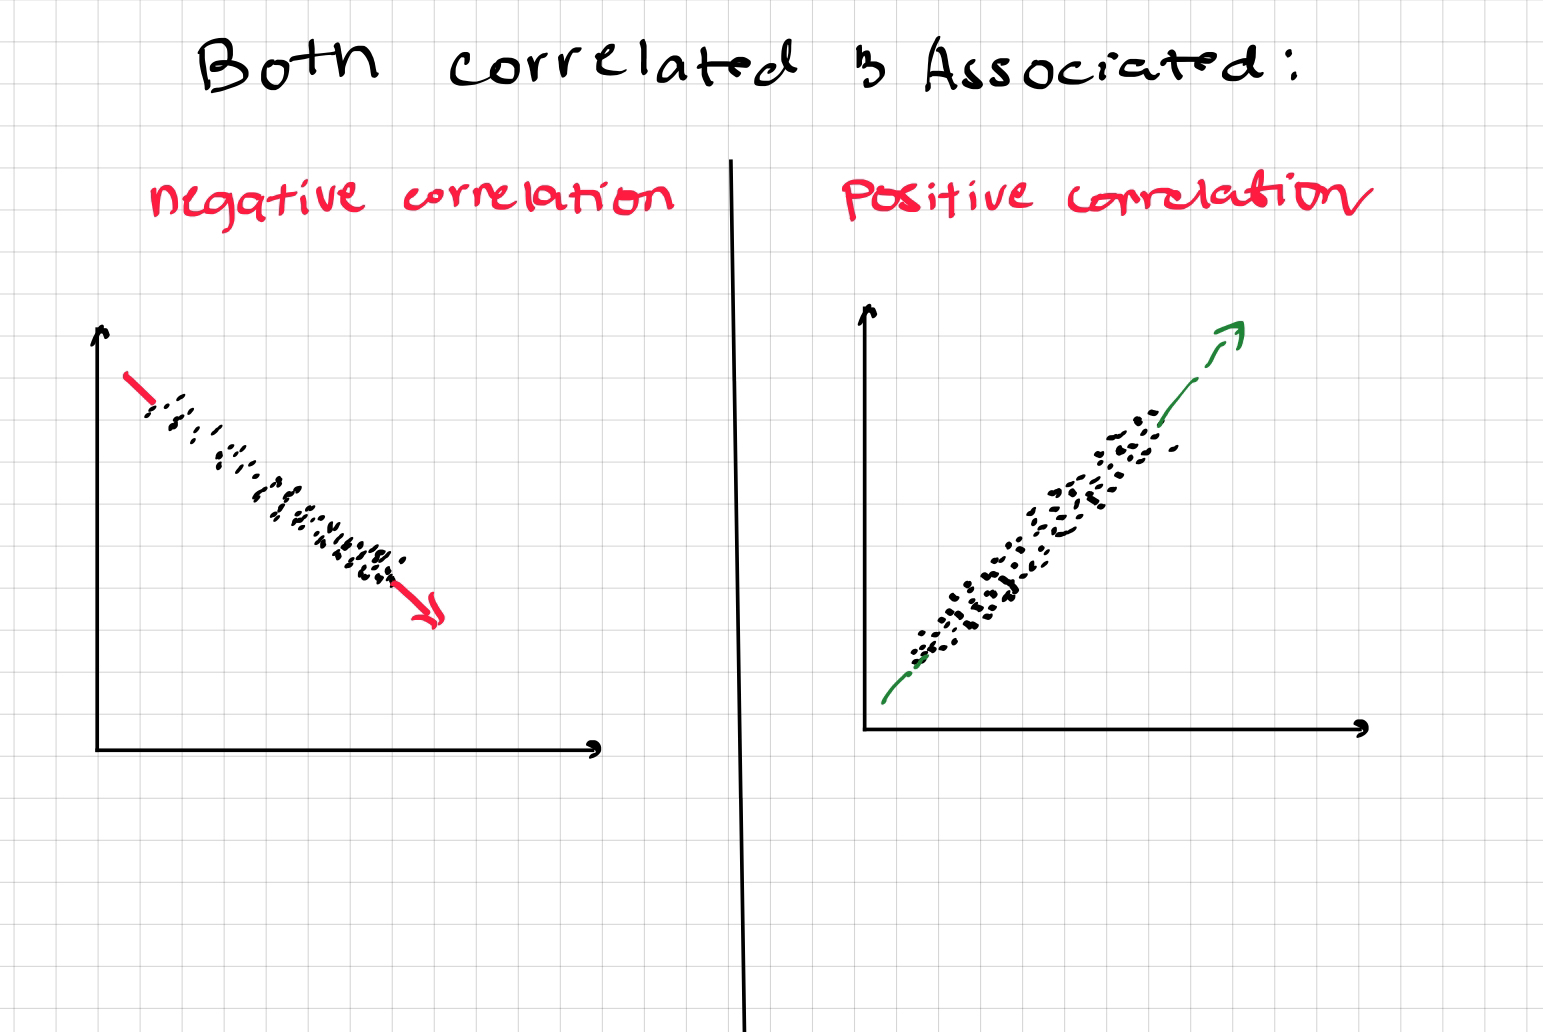
\includegraphics[width=10cm, keepaspectratio]{5a.png}

\easysubproblem{Give an example of two variables that are not correlated but are associated by drawing a plot.} \\ 
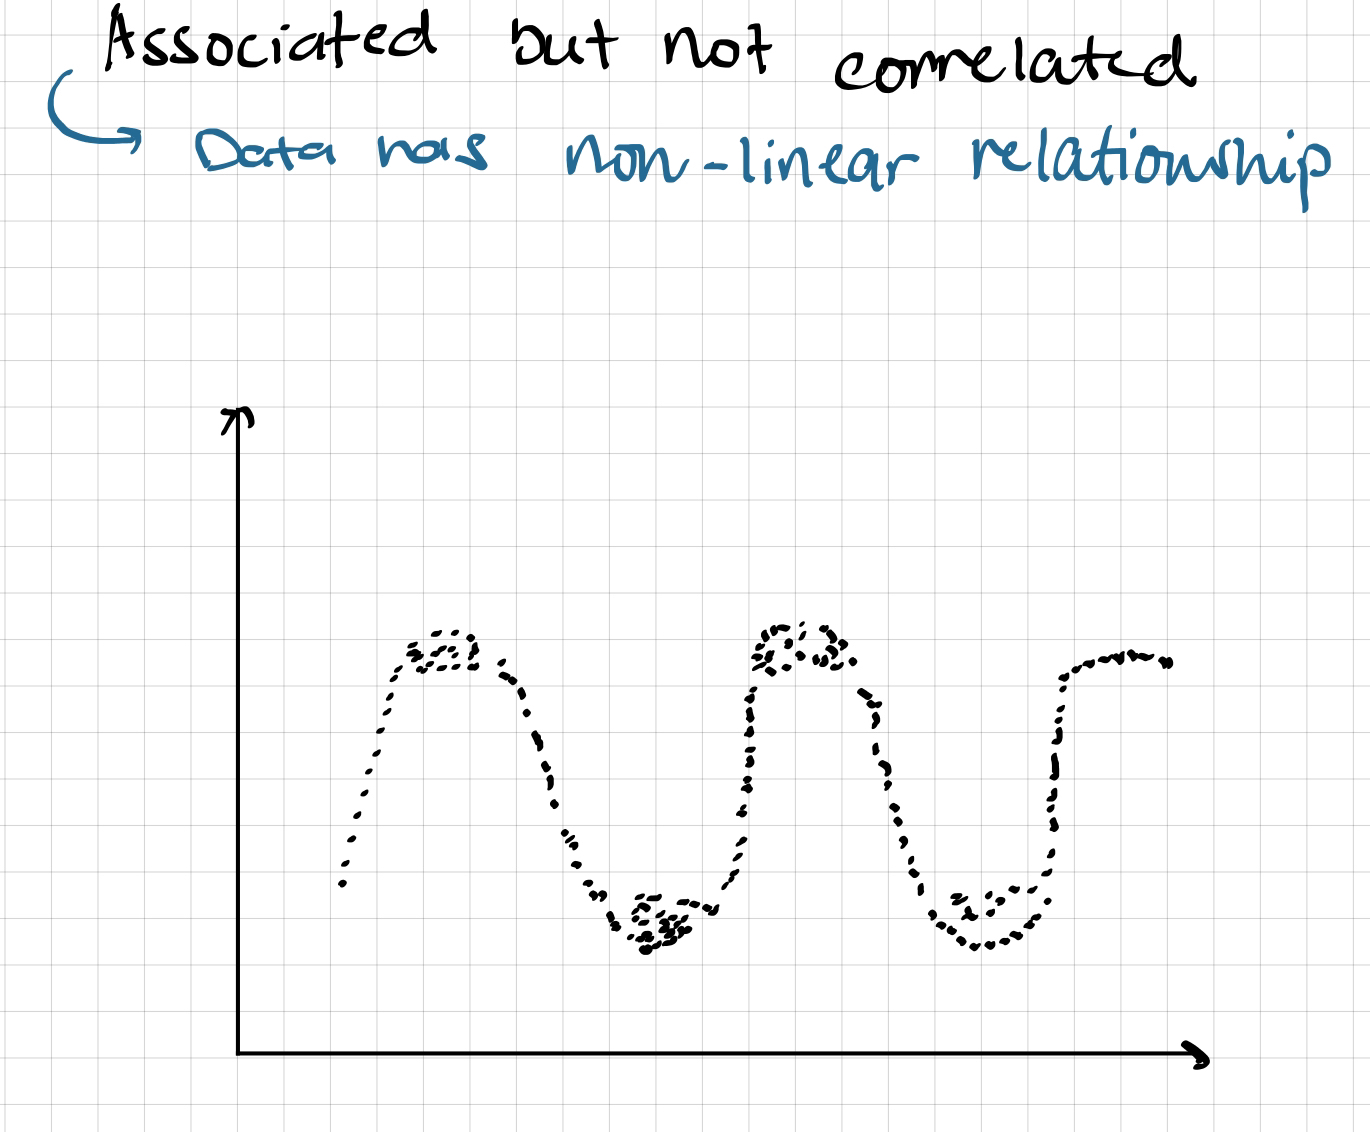
\includegraphics[width=10cm, keepaspectratio]{5b.png}

\newpage 
\easysubproblem{Give an example of two variables that are not correlated nor associated by drawing a plot.} \\ 
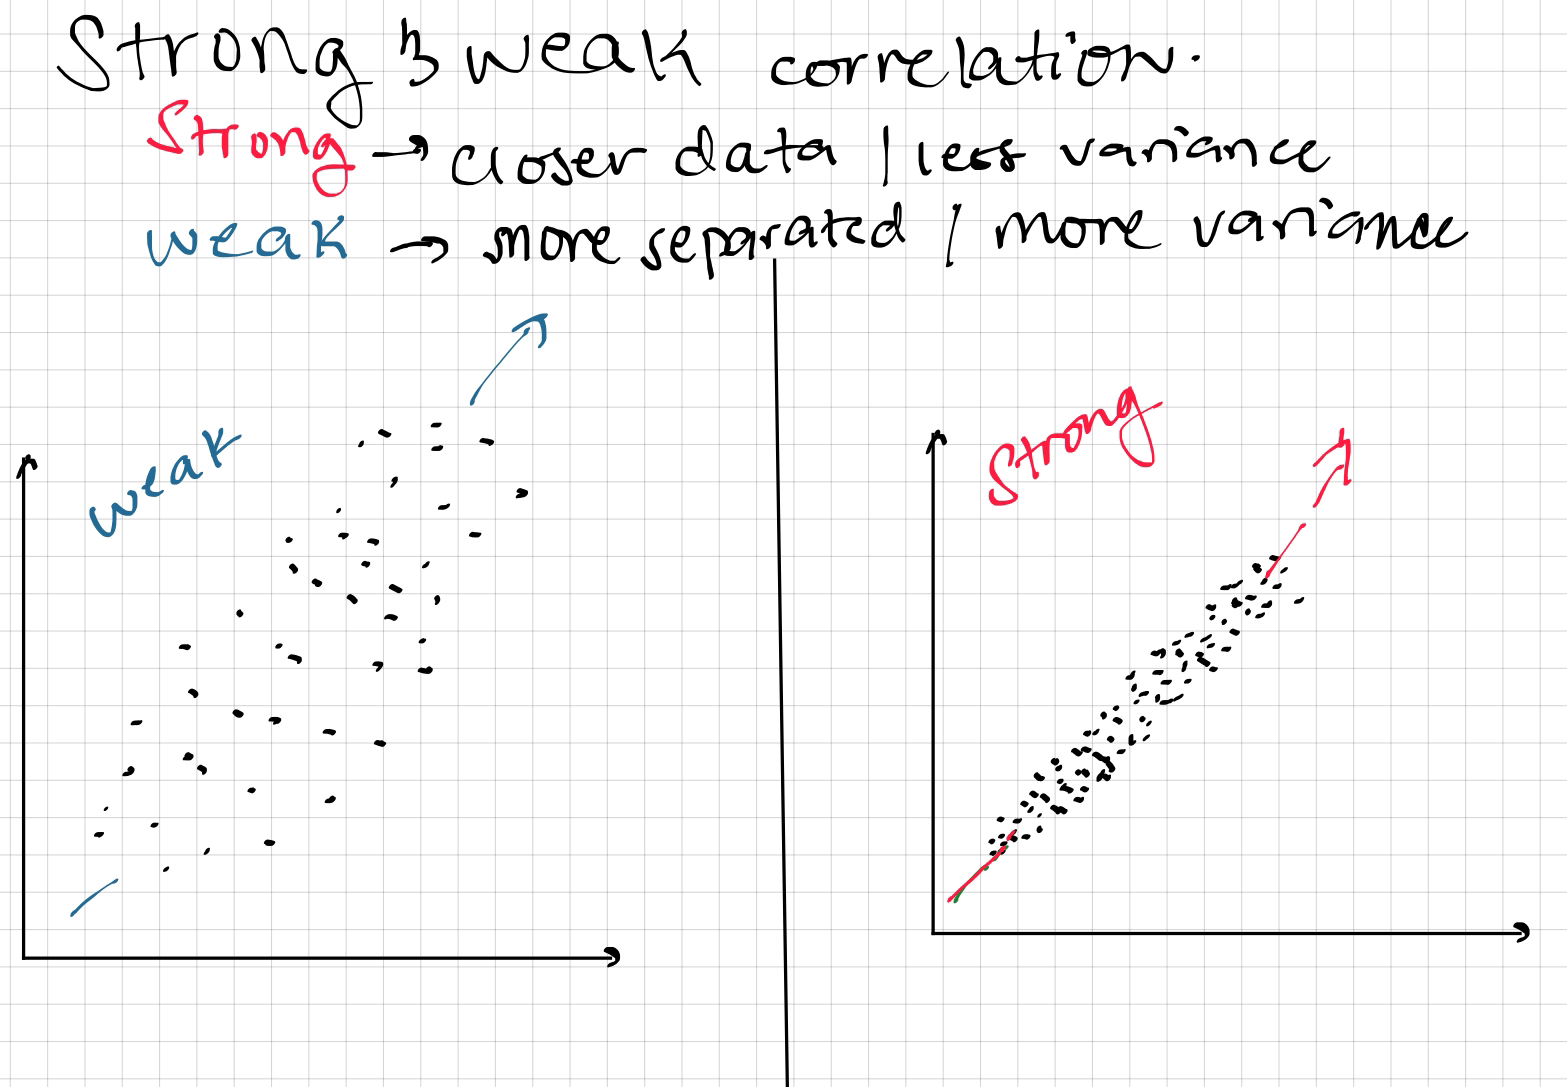
\includegraphics[width=10cm, keepaspectratio]{5c.png} 


\easysubproblem{Can two variables be correlated but not associated? Explain.} \\ 
\textbf{Answer: } \\ 

Two variables can be either both correlated and associated, or just associated. It is impossible for variables to be correlated but not associated, as correlation is a specific type of association. When two variables have a linear relationship, they are correlated, but if they have a non-linear relationship, they are merely associated. In summary, if two variables are either correlated or associated, they are related in some way. However, to say that they have a specific type of relationship but are not associated is incorrect because stating that they are correlated inherently implies that they are associated. \\ 

\end{enumerate}

\newpage 
\problem{These are questions about multivariate linear model fitting using the least squares algorithm.}

\begin{enumerate}

\hardsubproblem{Derive $\partialop{\c}{\c^\top A \c}$ where $\c \in \reals^n$ and $A \in \reals^{n \times n}$ but \textit{not} symmetric. Get as far as you can.} \\ 
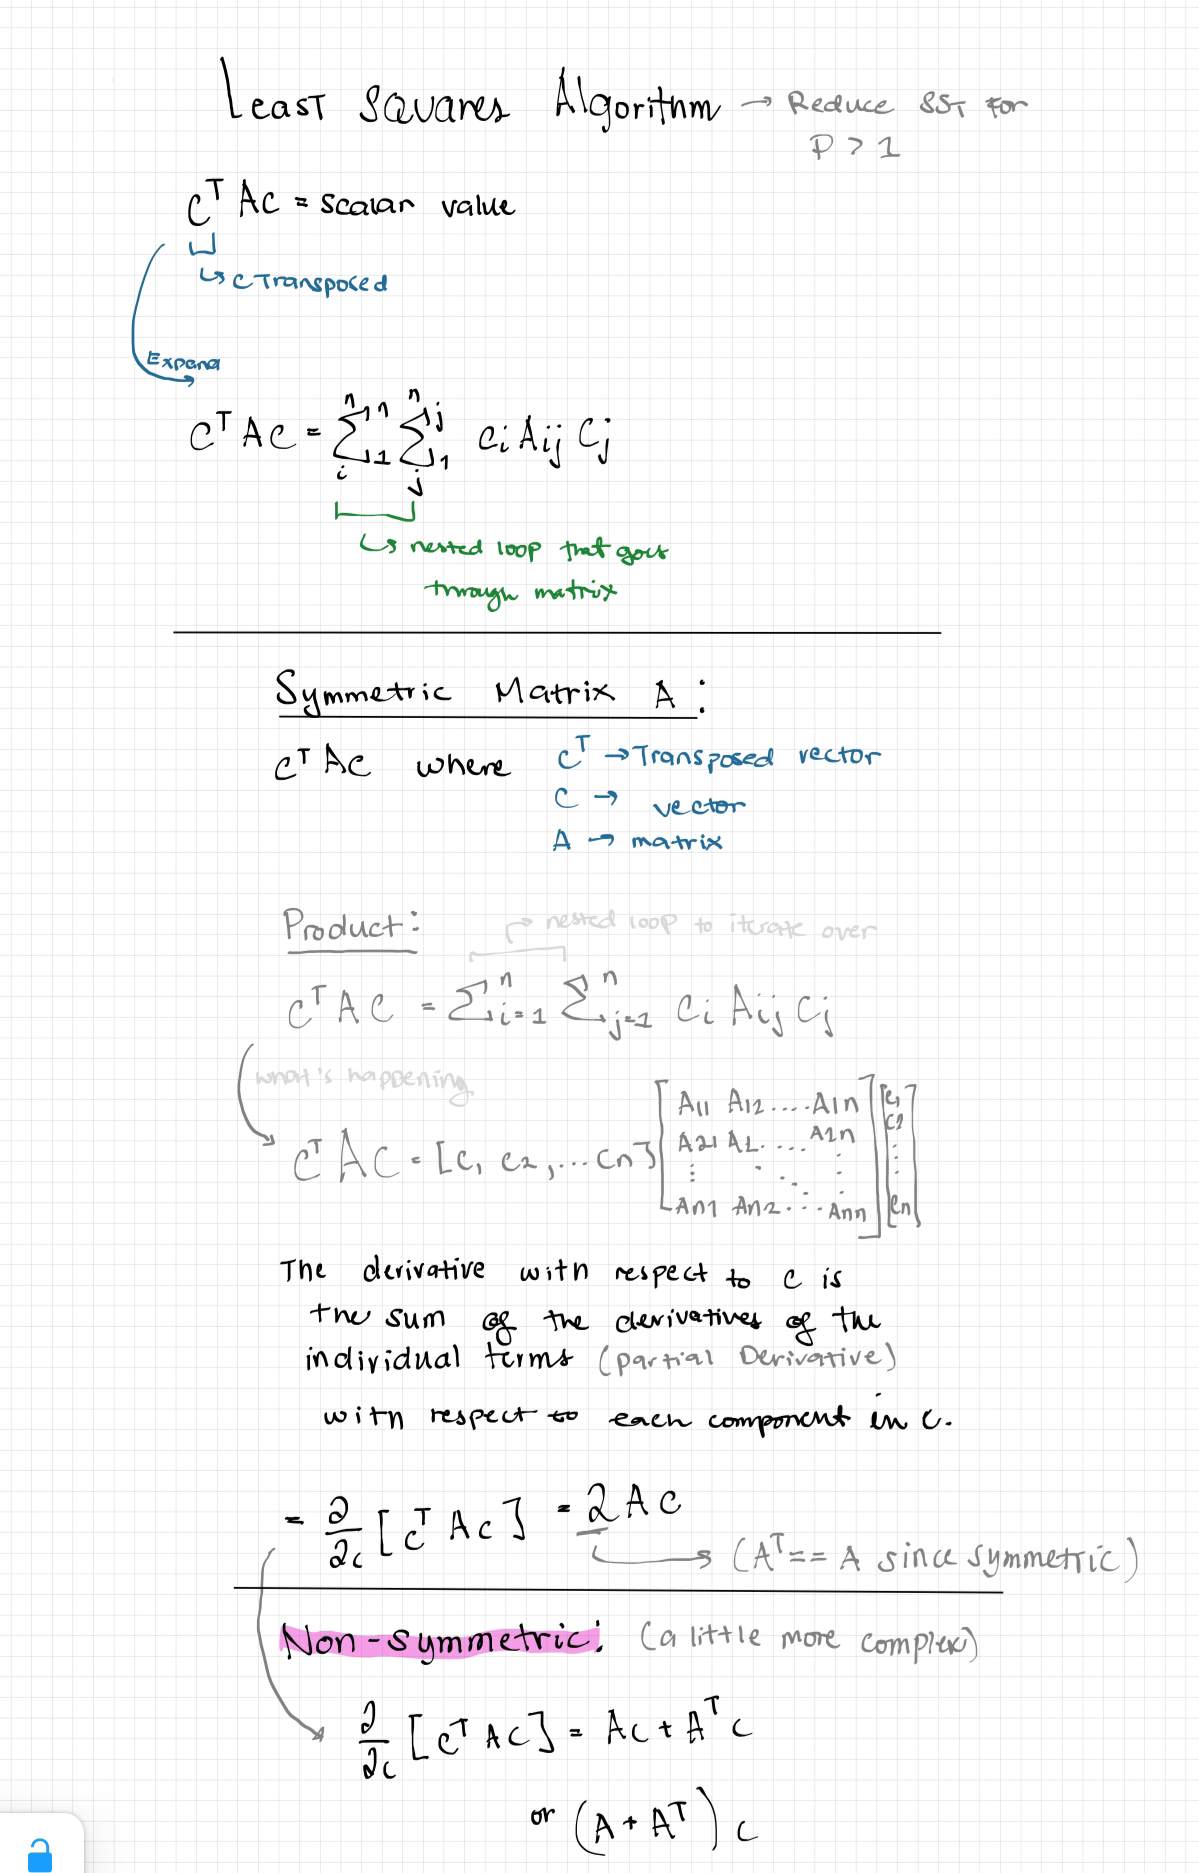
\includegraphics[width=10cm, keepaspectratio]{6a.png}

\easysubproblem{Given matrix $X \in \reals^{n \times (p+1)}$, full rank and first column consisting of the $\onevec_n$ vector, rederive the least squares solution $\b$ (the vector of coefficients in the linear model shipped in the prediction function $g$). No need to rederive the facts about vector derivatives.}\\
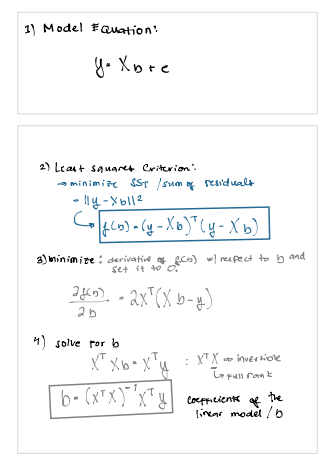
\includegraphics[width=10cm, keepaspectratio]{6b.png}

\intermediatesubproblem{Consider the case where $p = 1$. Show that the solution for $\b$ you just derived in (b) is the same solution that we proved for simple regression. That is, the first element of $\b$ is the same as $b_0 = \ybar - r \frac{s_y}{s_x}\xbar$ and the second element of $\b$ is $b_1 = r \frac{s_y}{s_x}$.}  \\ 


\easysubproblem{If $X$ is rank deficient, how can you solve for $\b$? Explain in English.} \\
\textbf{Answer: } \\ 
If \(X\) is rank deficient, this implies that the features in \(X\) are not linearly independent.
Therefore, we cannot use the normal equation \(b = (X^{\top}X)^{-1}X^{\top}y\) because \(X^{\top}X\) is not invertible,
meaning it does not have a unique inverse. Techniques such as Ridge Regression and Pseudo-Inverse
could be used to solve for \(b\). \\
\textbf{Citation: } \\ 
n/a (2024, February 25). \\
"Rank Deficiency Solutions". Retrieved from https://chat.openai.com/c/e5a24cde-c381-4122-a7d5-11aef6e17fe8 (ChatGPT)


\hardsubproblem{Prove $\rank{X} =\rank{X^\top X}$.}\\


%\hardsubproblem{Given matrix $X \in \reals^{n \times (p+1)}$, full rank and first column consisting of the $\onevec_n$ vector, now consider cost multiples (\qu{weights}) $c_1, c_2, \ldots, c_n$ for each mistake $e_i$. As an example, previously the mistake for the 17th observation was $e_{17} := y_{17} - \hat{y}_{17}$ but now it would be $e_{17} := c_{17} (y_{17} - \hat{y}_{17})$.  Derive the weighted least squares solution $\b$. No need to rederive the facts about vector derivatives. Hints: (1) show that SSE is a quadratic form with the matrix $C$ in the middle (2) Split this matrix up into two pieces i.e. $C = C^{\half} C^{\half}$, distribute and then foil (3) note that a scalar value equals its own transpose and (4) use the vector derivative formulas.}\spc{10}


\intermediatesubproblem{Prove that $g(\bracks{1 ~\xbar_1~ \xbar_2~ \ldots~ \xbar_p}) =\bar{y}$ in OLS.} \\
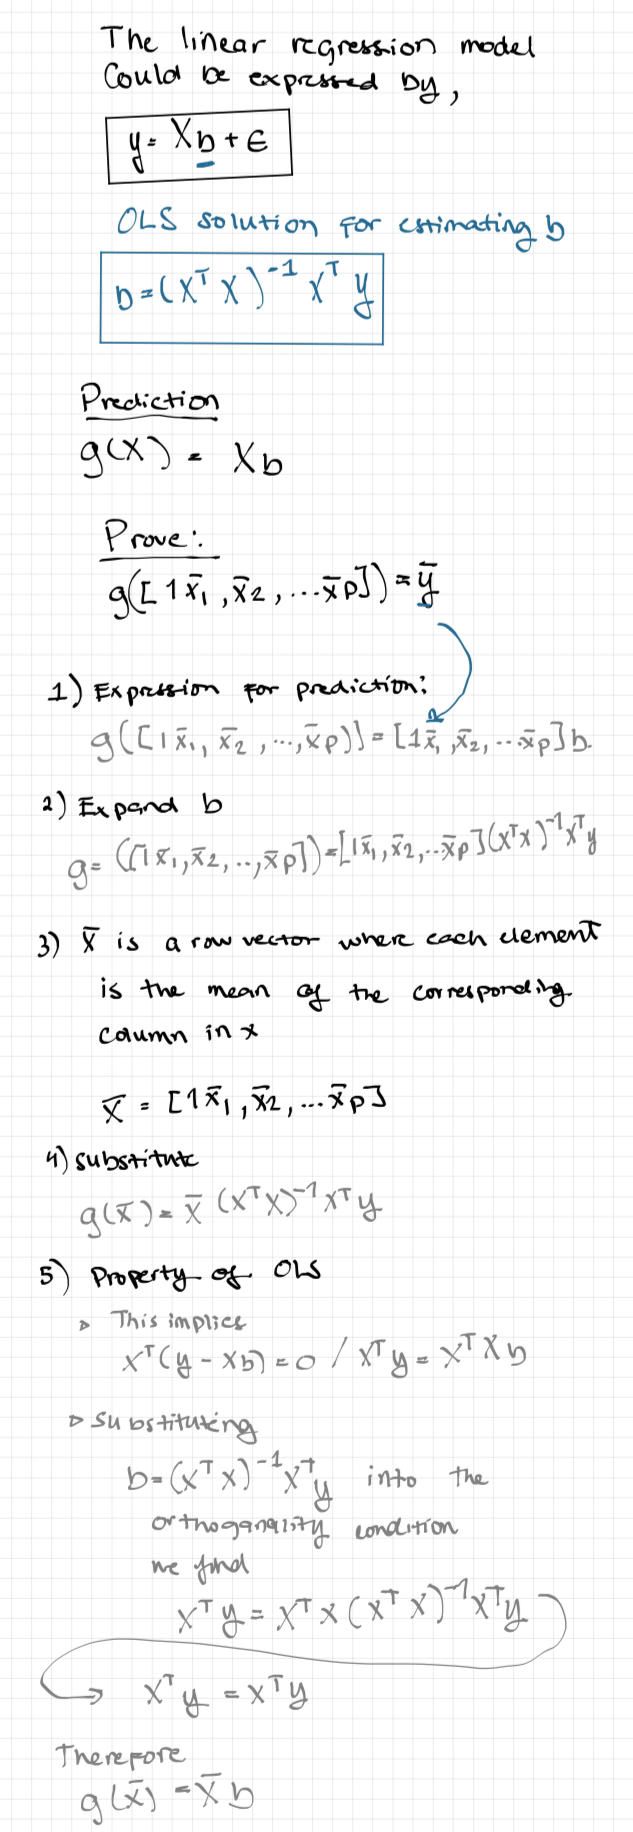
\includegraphics[width=8cm, keepaspectratio]{6f.png} \\ 
"OLS Properties Proof". Retrieved from https://chat.openai.com/c/b0f4defd-66e4-45d0-bef7-98e25a4978e3 (ChatGPT)


\intermediatesubproblem{Prove that $\bar{e} = 0$ in OLS.}\spc{10}

\hardsubproblem{If you model $\y$ with one categorical nominal variable that has levels $A, B, C$, prove that the OLS estimates look like $\ybar_A$ if $x = A$, $\ybar_B$ if $x = B$ and $\ybar_C$ if $x = C$. You can choose to use an intercept or not. Likely without is easier.}\spc{10}


\end{enumerate}



\end{document}

